% This file was created by matlab2tikz.
% Minimal pgfplots version: 1.3
%
%The latest updates can be retrieved from
%  http://www.mathworks.com/matlabcentral/fileexchange/22022-matlab2tikz
%where you can also make suggestions and rate matlab2tikz.
%
\documentclass[tikz]{standalone}
\usepackage{pgfplots}
\usepackage{grffile}
\pgfplotsset{compat=newest}
\usetikzlibrary{plotmarks}
\usepackage{amsmath}

\begin{document}
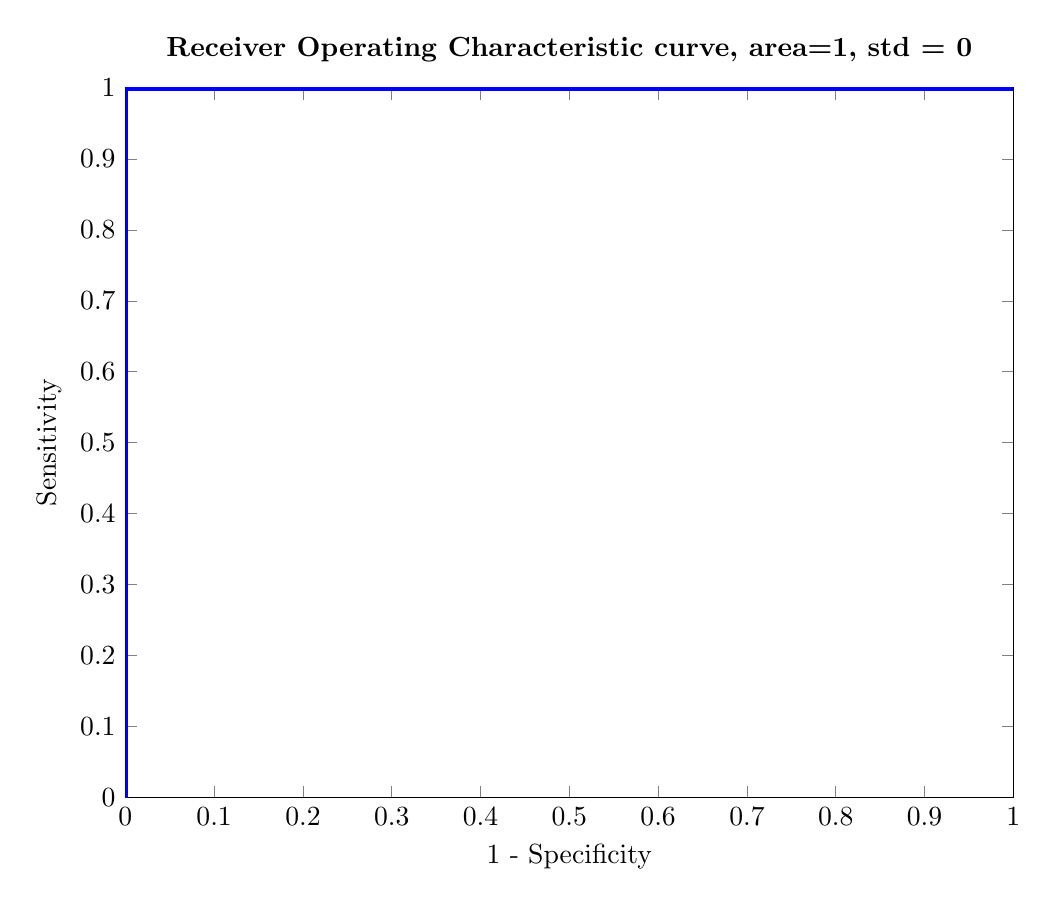
\begin{tikzpicture}

\begin{axis}[%
width=4.440104in,
height=3.548646in,
at={(0.744792in,0.478958in)},
scale only axis,
xmin=0,
xmax=1,
xlabel={1 - Specificity},
ymin=0,
ymax=1,
ylabel={Sensitivity},
title style={font=\bfseries},
title={Receiver Operating Characteristic curve, area=1, std = 0}
]
\addplot [color=blue,solid,line width=2.0pt,forget plot]
  table[row sep=crcr]{%
0	0\\
0	0.0666666666666667\\
0	0.133333333333333\\
0	0.2\\
0	0.266666666666667\\
0	0.333333333333333\\
0	0.4\\
0	0.466666666666667\\
0	0.533333333333333\\
0	0.6\\
0	0.666666666666667\\
0	0.733333333333333\\
0	0.8\\
0	0.866666666666667\\
0	0.933333333333333\\
0	1\\
0.2	1\\
0.4	1\\
0.6	1\\
0.8	1\\
1	1\\
};
\end{axis}
\end{tikzpicture}%
\end{document}